\documentclass{article}

\usepackage[left=2.5cm, right=2.5cm, top=2.5cm, bottom=2.5cm]{geometry}
\usepackage{amsmath}
\usepackage{listings}
\usepackage{color}
\usepackage{placeins}
\usepackage{graphicx}
\graphicspath{ {C:\Users\Dell\Documents\Graduate - Economics\Development Economics} }

\title{Economics of Development: Problem Set 1}
\author{S M Sajid Al Sanai}
\date{April 20, 2019}

\begin{document}

\maketitle
\pagenumbering{arabic}
\tableofcontents

\lstset{
	frame=lines,
	basicstyle=\small\sffamily,
	tabsize=4,
	columns=fixed,
	showstringspaces=false,
	showtabs=false,
	keepspaces,
	commentstyle=\color{red},
	keywordstyle=\color{blue}
}

\newpage

\section{Question II}

\subsection{Source}

\lstinputlisting{PS1_SMSajidAlSanai.do}

\newpage

\subsection{Output}

\lstinputlisting{PS1_SMSajidAlSanai.txt}

\newpage

\subsection{Graphs}

\begin{figure}[h]
  \centering
    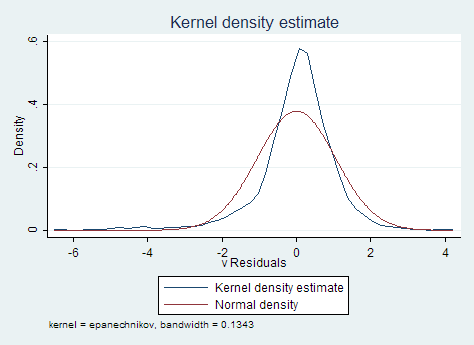
\includegraphics[width=1.0\textwidth]{graph1}
\end{figure}
\FloatBarrier

\begin{figure}[h]
  \centering
    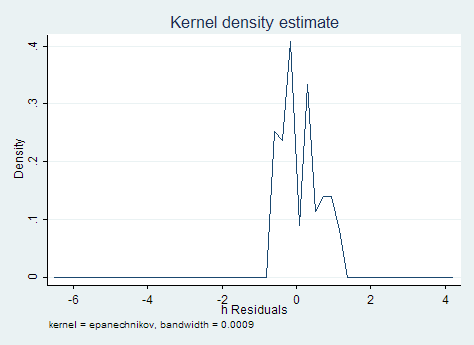
\includegraphics[width=1.0\textwidth]{graph2}
\end{figure}
\FloatBarrier

\begin{figure}[h]
  \centering
    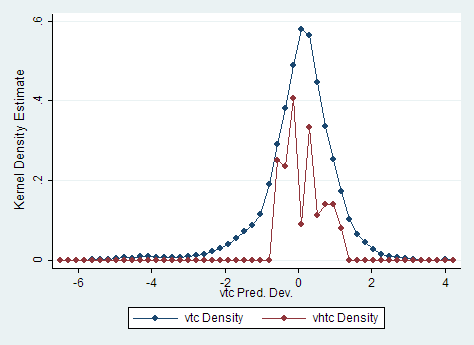
\includegraphics[width=1.0\textwidth]{graph3}
\end{figure}
\FloatBarrier

\end{document}